\documentclass[12pt]{exam}

% essential packages
\usepackage{fullpage} % margin formatting
\usepackage{enumitem} % configure enumerate and itemize
\usepackage{amsmath, amsfonts, amssymb, mathtools} % math symbols
\usepackage{xcolor, colortbl} % colors, including in tables
\usepackage{makecell} % thicker \Xhline in table
\usepackage{graphicx} % images, resizing
\usepackage{tikz} % drawing graphs
\usepackage{algpseudocode}
\usetikzlibrary{positioning}

% paragraph formatting
\setlength{\parskip}{6pt}
\setlength{\parindent}{0cm}

% newline after Solution:
\renewcommand{\solutiontitle}{\noindent\textbf{Solution:}\par\noindent}

% less space before itemize/enumerate
\setlist{topsep=0pt}

% creates \filcl to grey out cells for groupwork grading
\newcommand{\filcl}{\cellcolor{gray!25}}

% creates \probnum to get the problem number
\newcounter{probnumcount}
\setcounter{probnumcount}{1}
\newcommand{\probnum}{\arabic{probnumcount}. \addtocounter{probnumcount}{1}}

% use roman numerals by default
\setlist[enumerate]{label={(\roman*)}}

% creates custom list environments for grading guidelines, question parts
\newlist{guidelines}{itemize}{1}
\setlist[guidelines]{label={}, left=0pt .. \parindent, nosep}
\newlist{gwguidelines}{enumerate}{1}
\setlist[gwguidelines]{label={(\roman*)}, nosep}
\newlist{qparts}{enumerate}{2}
\setlist[qparts]{label={(\alph*)}}
\newlist{qsubparts}{enumerate}{2}
\setlist[qsubparts]{label={(\roman*)}}
\newlist{stmts}{enumerate}{1}
\setlist[stmts]{label={(\roman*)}, nosep}
\newlist{pflist}{itemize}{4}
\setlist[pflist]{label={$\bullet$}, nosep}
\newlist{enumpflist}{enumerate}{4}
\setlist[enumpflist]{label={(\arabic*)}, nosep}

\printanswers

\begin{document}
%%%%%%%%%%%%%%% TITLE PAGE %%%%%%%%%%%%%%%
\title{EECS 203: Discrete Mathematics\\
  Fall 2023\\
  Homework 11}
\date{}
\author{}
\maketitle
\vspace{-50pt}
\begin{center}
  \huge Due \textbf{Tuesday, December 5}, 10:00 pm\\
\Large No late homework accepted past midnight.\\
\vspace{10pt}
\large Number of Problems: $9+2$
\hspace{3cm}
Total Points: $100+18$
\end{center}
\vspace{25pt}
\begin{itemize}
    \item \textbf{Match your pages!} Your submission time is when you upload the file, so the time you take to match pages doesn't count against you.
    \item Submit this assignment (and any regrade requests later) on Gradescope. 
    \item Justify your answers and show your work (unless a question says otherwise).
    \item By submitting this homework, you agree that you are in compliance with the Engineering Honor Code and the Course Policies for 203, and that you are submitting your own work.
    \item Check the syllabus for full details.
\end{itemize}
\newpage
%%%%%%%%%%%%%%% TITLE PAGE %%%%%%%%%%%%%%% 


\section*{Individual Portion}


\textbf{Reminder: }Make sure to leave your answers in combination, permutation, or factorial form and \textbf{not} simplified.

\subsection* {\probnum Bayes Easy [12 points]}

Suppose that one person in 10,000 people has a rare genetic disease. There is an excellent test for the disease; 99.9\% of people with the disease test positive and only 0.02\% who do not have the disease test positive.

\begin{qparts}
    \item What is the probability that someone who tests positive has the genetic disease?
    \item What is the probability that someone who tests negative does not have the disease?
\end{qparts}

\begin{solution}
    ~\\~\\~\\~\\~\\~\\~\\~\\~\\~\\~\\~\\~\\~\\~\\~\\~\\~\\~\\~\\~\\~\\~\\~\\~\\~\\~\\~\\
\end{solution}

\subsection*{\probnum Spaced Out [12 points]}
A space probe heading to Mars sends messages back to Earth using bit strings. Suppose that it sends a `1' one-third of the time and a `0' two-thirds of the time. However, the communication channel is noisy---when a 1 is sent, it is possible that noise interferes, causing Earth to receive a 0 and vise versa. Probabilities of different situations are listed: 
\begin{itemize}
    \item When a 0 is sent, the probability that it is received correctly is 0.6.
    \item When a 0 is sent, the probability that it is received incorrectly (as a 1) is 0.4.
    \item When a 1 is sent, the probability that it is received correctly is 0.8.
    \item When a 1 is sent, the probability that it is received incorrectly (as a 0) is 0.2.
\end{itemize}
\begin{qparts}
    \item Suppose Earth received a `0'.  What is the probability that the probe sent `0'?
    \item The space probe then transmits the same bit as part (a) again, and Earth receives `0' a second time. What is the probability the probe sent a 0? You can assume that the event of a bit getting corrupted is independent of any other bit getting corrupted.
\end{qparts}
    
\begin{solution}
    ~\\~\\~\\~\\~\\~\\~\\~\\~\\~\\~\\~\\~\\~\\~\\~\\~\\
    ~\\~\\~\\~\\~\\~\\~\\~\\~\\~\\~\\~\\~\\~\\~\\~\\~\\~\\~\\~\\~\\~\\~\\~\\~\\~\\~\\~\\
\end{solution}

\subsection*{\probnum Aye Aye Esti-matey [8 points]} 
Give the tightest big-$O$ estimate of the following functions:
\begin{qparts}
    \item $g(n) = (3^n)\cdot (n^2 + \log n)\cdot(2n^4+n) + (4n + n!)\cdot(1000^{n+1000} + n^n)$
    \item $f(n) = (n^2 + n\log n)\cdot\left(4n + \sum\limits_{i=1}^{10} n^i\right)$
\end{qparts}
\textbf{Note:} $\sum\limits_{i=1}^{10} n^i = n^1+n^2+n^3+\dots+n^{10}$

\begin{solution}
    ~\\~\\~\\~\\~\\~\\~\\
    ~\\~\\~\\~\\~\\~\\~\\~\\~\\~\\~\\~\\~\\~\\~\\~\\~\\~\\~\\~\\~\\~\\~\\~\\~\\~\\~\\~\\
\end{solution}

\subsection*{\probnum Al Gore, It Him [12 points]}
Give a big-$O$ estimate for the number of operations, where an operation is an addition or a multiplication, used in this segment of an algorithm (ignoring comparisons used to test the conditions in the {\bf while} or \textbf{for} loop).

\textbf{Hint:} Your estimates may use more than one variable.

\begin{qparts}
    \item \begin{algorithmic}
        \State{$t\gets 0$}
        \For{$i\coloneqq 1\text{ to }n$}
            \For{$j\coloneqq 1\text{ to }m$}
                \State{$t\gets t+i+j$}
            \EndFor
        \EndFor
    \end{algorithmic}

    \item \begin{algorithmic}
        \State{$t\gets 0$}
        \For{$i\coloneqq 1\text{ to }n$}
            \State{$t\gets t\cdot 2$}
        \EndFor
        \For{$j\coloneqq 1\text{ to }m$}
            \State{$t\gets t+j$}
        \EndFor
    \end{algorithmic}

    \item \begin{algorithmic}
        \State{$t\gets 0$}
        \State{$i\gets 1$}
        \While{$i\le n$}
            \State{$t\gets t-i$}
            \State{$i\gets i\cdot 3$}
        \EndWhile
    \end{algorithmic}
\end{qparts}

\begin{solution}
    ~\\~\\~\\~\\~\\~\\~\\~\\~\\~\\
    ~\\~\\~\\~\\~\\~\\~\\~\\~\\~\\~\\~\\~\\~\\~\\~\\~\\~\\~\\~\\~\\~\\~\\~\\~\\~\\~\\~\\
\end{solution}


\subsection*{\probnum Breakout Room [12 points]}
In a class with 34 students there are 6 breakout rooms, with 3, 3, 4, 7, 8, and 9 students in each room, respectively.

\begin{qparts}
    \item Suppose we pick a room at random, and consider $X$ to be the random variable defined by the number of people in that room. What is the expected value of $X$?
    \item Now suppose we pick one of the students at random. Let $Y$ be the random variable defined by the number of people in that student's room. What is the expected value of $Y$?
\end{qparts}
\begin{solution}
    ~\\~\\~\\~\\~\\~\\~\\~\\~\\~\\
    ~\\~\\~\\~\\~\\~\\~\\~\\~\\~\\~\\~\\~\\~\\~\\~\\~\\~\\~\\~\\~\\~\\~\\~\\~\\~\\~\\~\\
\end{solution}


\subsection* {\probnum Rolling Dice [12 points]}
You roll a fair six-sided die 12 times. Find the probability that:
\begin{qparts}
    \item Exactly two rolls come up as a 6.
    \item Exactly two rolls come up as a 4, given that the first four rolls each came up as 3.
    \item At least two rolls come up as a 6.
\end{qparts}

\begin{solution}
    ~\\~\\~\\~\\~\\~\\~\\~\\~\\~\\~\\~\\~\\~\\~\\~\\~\\~\\~\\~\\~\\~\\~\\~\\~\\~\\~\\~\\
\end{solution}


\subsection*{\probnum More Dice [10 points]}
Suppose Emily is rolling a pair of standard dice until the dice roll sums to 8 three times. What is the probability that they will roll more than 4 times?

For example, some sequences of rolls include:
$$(1,2),(4,6),\underline{(4,4)},\underline{(5,3)},(2,5),(2,3),\underline{(6,2)}$$
$$\underline{(4,4)},(2,1),(4,5),(6,6),\underline{(5,3)}, (4,3),(5,5),\underline{(4,4)}$$

\begin{solution}
    ~\\
    ~\\~\\~\\~\\~\\~\\~\\~\\~\\~\\~\\~\\~\\~\\~\\~\\~\\~\\~\\~\\~\\~\\~\\~\\~\\~\\~\\~\\
\end{solution}

\subsection*{\probnum Mystery Boba [10 points]}
Isabel loves to get bubble tea on campus. On any given day, there is $15\%$ chance she gets taro milk tea, $25\%$ chance she gets a matcha latte, $40\%$ chance she gets passion fruit tea, and $20\%$ chance she doesn't get any bubble tea. Assume Isabel has a maximum of one bubble tea every day. 
\begin{qparts}
    \item In a 7-day week, what is the probability that Isabel gets 2 taro milk teas, 1 matcha latte, and 2 passion fruit teas (in any order)?
    \item In a 7-day week, what is the probability that Isabel gets exactly 4 passion fruit teas?
    \item Over 14-days, what is the expected number of taro milk teas Isabel gets?
    
\end{qparts}

\begin{solution}
    ~\\~\\~\\~\\~\\~\\~\\~\\~\\~\\
    ~\\~\\~\\~\\~\\~\\~\\~\\~\\~\\~\\~\\~\\~\\~\\~\\~\\~\\~\\~\\~\\~\\~\\~\\~\\~\\~\\~\\
\end{solution}


\subsection*{\probnum The 101 Dalmations Binary Ballet [12 points]}
Consider a binary sequence of length $14$ selected at random.  What is the expected number of times $101$ appears in the sequence? For example, it appears 4 times in the string 
$$\overline{10\underline{1}}\underline{01}0000\overline{10\underline{1}}\underline{01}.$$

\begin{solution}
    ~\\~\\~\\~\\~\\~\\~\\~\\~\\~\\
    ~\\~\\~\\~\\~\\~\\~\\~\\~\\~\\
    ~\\~\\~\\~\\~\\~\\~\\~\\~\\~\\
    ~\\~\\~\\~\\~\\~\\~\\~\\~\\~\\

\end{solution}


\pagebreak
\setcounter{probnumcount}{1}
\section*{Groupwork}
\subsection*{\probnum Grade Groupwork 10}
Using the solutions and Grading Guidelines, grade your Groupwork 10:
\begin{itemize}
    \item Mark up your past groupwork and submit it with this one.
    \item Write whether your submission achieved each rubric item. If it didn't achieve one, say why not.
    \item Use the table below to calculate scores.
    \item For extra credit, write positive comment(s) about your work.
    \item You don't have to redo problems correctly, but it is recommended!
    \item What if my group changed? \begin{itemize}
        \item If your current group submitted the same groupwork last time, grade it together.
        \item  If not, grade your version, which means submitting this groupwork assignment separately. You may discuss grading together.
    \end{itemize}
\end{itemize}

\begin{center}
\resizebox{\textwidth}{!}{\begin{tabular}{| c | c | c | c | c | c | c | c | c | c | c | c | c |}
\hline
 & (i) & (ii) & (iii) & (iv) & (v) & (vi) & (vii) & (viii) & (ix) & (x) & (xi) & Total:\\
\hline
Problem 2 & & & & & &\filcl &\filcl &\filcl &\filcl & \filcl& \filcl& \hspace{1cm}/15\\
\hline

Problem 3 & & & & & & \filcl& \filcl &\filcl &\filcl & \filcl& \filcl& \hspace{1cm}/15\\
\Xhline{1.25pt}
Total: &\filcl &\filcl &\filcl &\filcl &\filcl &\filcl &\filcl &\filcl & \filcl& \filcl& \filcl&\hspace{1cm}/30\\
\hline
\end{tabular}}
\end{center}

\clearpage

\subsection*{Previous Groupwork 10(1): Lily's Lily Pads [15 points]}
Lily the Frog is on a lily pad and wants to get to her home! She can jump from lily pad to lily pad to help reach this goal. The lily pads are arranged in a grid. Lily starts on the \textbf{bottom-left} lily pad, and her home is at the \textbf{top-right} lily pad. Lily can only move one lily pad \textbf{upward} or one lily pad \textbf{rightward} at a time.\\

Each lily pad has coordinates of the form $(x, y) \in \mathbb{N} \times \mathbb{N}$, where $x$ represents how far rightward a point is from the left of the grid, and $y$ represents how far upward a point is from the bottom of the grid. Lily starts at location $(0, 0)$, and her home is at location $(x_H, y_H)  \in \mathbb{N} \times \mathbb{N}$.\\

\begin{center}
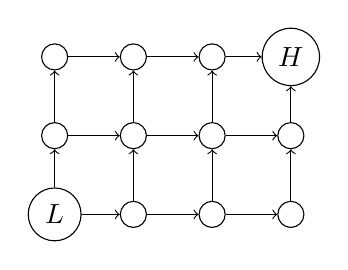
\begin{tikzpicture}[main/.style = {draw, circle}]
    \node[main] (1) {$L$};
    \node[main] (2) [above of=1] {};
    \node[main] (3) [above of=2] {};
    \node[main] (4) [right of=1] {};
    \node[main] (5) [above of=4] {};
    \node[main] (6) [above of=5] {};
    \node[main] (7) [right of=4] {};
    \node[main] (8) [above of=7] {};
    \node[main] (9) [above of=8] {};
    \node[main] (10) [right of=7] {};
    \node[main] (11) [above of=10] {};
    \node[main] (12) [above of=11] {$H$};
    \draw[->] (1) -- (2);
    \draw[->] (1) -- (4);
    \draw[->] (2) -- (3);
    \draw[->] (2) -- (5);
    \draw[->] (3) -- (6);
    \draw[->] (4) -- (5);
    \draw[->] (4) -- (7);
    \draw[->] (5) -- (6);
    \draw[->] (5) -- (8);
    \draw[->] (6) -- (9);
    \draw[->] (7) -- (8);
    \draw[->] (7) -- (10);
    \draw[->] (8) -- (9);
    \draw[->] (8) -- (11);
    \draw[->] (9) -- (12);
    \draw[->] (10) -- (11);
    \draw[->] (11) -- (12);
\end{tikzpicture}
\end{center}

In the above example, $(x_H, y_H) = (3, 2)$. In the general case, though, $(x_H, y_H)$ could be any ordered pair of natural numbers.

\begin{qparts}
    \item How many different paths can Lily take to get home?
    \item Lily's frog friend, Francine, is also on the grid at coordinates $(x_F, y_F) \in \mathbb{N} \times \mathbb{N}$ such that $0 \leq x_F \leq x_H$ and $0 \leq y_F \leq y_H$. What is the probability that Lily meets Francine on her path home? You may assume that any two paths home are equally likely for Lily to take.
\end{qparts}
\begin{solution}
    ~\\~\\~\\~\\~\\~\\~\\~\\~\\~\\~\\~\\~\\~\\~\\~\\~\\~\\~\\~\\~\\~\\~\\~\\~\\~\\~\\~\\
    ~\\~\\~\\~\\~\\~\\~\\~\\~\\~\\~\\~\\~\\~\\~\\
\end{solution}

\subsection*{Previous Groupwork 10(2) Random Connections [15 points]}
We say that a \textit{random graph} is an undirected graph where, for each pair of vertices, there is an independent $\frac{1}{3}$ chance that they are adjacent. It's a bit like Lily's pond, except that the vertices aren't in a grid, and you can move in any direction.

We want to learn about the connectedness of random graphs.

Let $G$ be a finite random graph. Let's split the vertices into two nonempty sets, $A, B \subseteq V$.

\begin{qparts}
    \item Let $a \in A$. What is the probability that no element of $B$ is adjacent to $a$?
    \item What is the probability that there is some $a \in A$ and $b \in B$ such that $a$ is adjacent to $b$?
    \item Let's imagine doing this with larger and larger graphs. Define $f(a, b)$ be your answer to the previous problem when $|A| = a$ and $|B| = b$. What is
    \[ \lim_{a+b \to \infty} f(a,b)? \]
    \item This isn't quite a proof, but your answer to (c) might lead you to some ideas. What might you conjecture about the connectedness of infinite random graphs?
\end{qparts}
\begin{solution}
    ~\\~\\~\\~\\~\\~\\~\\~\\~\\~\\~\\~\\~\\~\\~\\~\\~\\~\\~\\~\\~\\~\\~\\~\\~\\~\\~\\~\\
    ~\\~\\~\\~\\~\\~\\~\\~\\
\end{solution}

\subsection*{\probnum I Am Speed [10 points]}
Suppose we have two algorithms, $\mathcal A$ and $\mathcal B$.  Suppose that on inputs of size $n$, algorithm $\mathcal A$ runs in time $\Theta(n^2)$, while algorithm $\mathcal B$ runs in time $\Theta(n^3)$. Show that there exists some $n_0$ such that for any $n > n_0$, algorithm $\mathcal A$ will take less time to run than algorithm $\mathcal B$ on inputs of size $n$.\\
\textbf{Note:} you may find it useful for your notation to let the runtime of $\mathcal A$ on inputs of size n be denoted as $f_{\mathcal A}(n)$, and similarly for algorithm $\mathcal B$ as $f_{\mathcal B}(n)$.

\begin{solution}
    ~\\~\\~\\~\\~\\~\\~\\~\\~\\~\\~\\~\\~\\~\\~\\~\\~\\~\\~\\~\\~\\~\\~\\~\\~\\~\\~\\~\\
    ~\\~\\~\\~\\~\\~\\~\\~\\
\end{solution}


\subsection*{\probnum GameStop or GameRoll? [8 points]}
In a game of repeated die rolls, a player is allowed to roll a standard die up to $n$ times, where $n$ is determined prior to the start of the game. On any roll except the last, the player may choose to either keep that roll as their final score, or continue rolling in hopes of a higher roll later on. If the player rolls all $n$ times, then on the $n$-th roll the player must keep that roll as their final score. A player always acts to maximize their expected final score. Finally, let $V_n$ denote the final score in a game with a max of $n$ rolls allowed.
\begin{qparts}
    \item Compute $E(V_2)$ with justification.
    \item Compute $E(V_3)$ with justification.
    \item Find the smallest $n$ such that $E(V_n) \geq 5$.
\end{qparts}

\begin{solution}
    ~\\~\\~\\~\\~\\~\\~\\~\\~\\~\\~\\~\\~\\~\\~\\~\\~\\~\\~\\~\\~\\~\\~\\~\\~\\~\\~\\~\\
    ~\\~\\~\\~\\~\\~\\~\\~\\~\\~\\~\\~\\~\\~\\~\\
\end{solution}

\end{document}
